\documentclass[10pt]{article}

\usepackage{fullpage}
\usepackage{graphics}
\usepackage{natbib}
\usepackage{amssymb,amsthm,amsmath}

\newtheorem{proposition}{Proposition}
\newtheorem{lemma}[proposition]{Lemma}
\newtheorem{corollary}[proposition]{Corollary}
\newtheorem{theorem}[proposition]{Theorem}

\renewcommand{\P}{\mathcal{P}}
\newcommand{\indicator}[1]{\mathbf{1}\left[{#1}\right]}
\newcommand{\x}{\mathbf{x}}

\DeclareMathOperator{\argmin}{argmin}
\DeclareMathOperator{\err}{err}
\DeclareMathOperator{\Exp}{\mathbf{E}}


\begin{document}

\title{Semi-supervised learning: The value of unlabeled data}
\author{Alexander Golovnev \and D\'avid P\'al \and Bal\'azs Sz\"or\'enyi}

\maketitle

\begin{abstract}
We show a separation of labeled sample complexity between learning \emph{with}
and \emph{without} the knowledge of the distribution of the unlabeled data. For
the class of projections over the boolean hypercube of dimension $n$, we show a
separation by $\Theta(\log n)$ multiplicative factor.

Learning with the knowledge of the distribution (a.k.a. \emph{fixed-distribution
learning}) can be viewed as an idealized scenario of semi-supervised learning
where the number of unlabeled data points is so great that the unlabeled
distribution is known almost exactly. For this reason, we call the separation
the \emph{value of unlabeled data}.
\end{abstract}


\section{Realizable Case: Projections}

\cite{Hanneke-2016} showed that for any class $C$ of Vapnik-Chervonenkis
dimension $d$ there exists an algorithm that $\epsilon$-learns any target
function under any domain distribution  from $O\left(\frac{d +
\log(1/\delta)}{\epsilon}\right)$ examples with probability at least $1-\delta$.
On the other hand, for any algorithm and any class $C$ of Vapnik-Chervonenkis dimension
$d \ge 2$ and any $\epsilon \in (0,1)$ and $\delta \in (0,1)$ there exists a
distribution over the domain and a concept which requires at least $\Omega
\left(\frac{d + \log(1/\delta)}{\epsilon}\right)$ examples to $\epsilon$-learn
with probability at least $1 - \delta$; see~\cite[Theorem
5.3]{Anthony-Bartlett-1999} or \cite{Blumer-Ehrenfeucht-Haussler-Warmuth-1989,
Ehrenfeucht-Haussler-Kearns-Valiant-1989}.

The proof of the lower bound constructs a distribution that does \emph{not}
depend on the algorithm. (The distribution is a fixed distribution over a
fixed set shattered by $C$.) So even an algorithm that ``knows'' (``is tailored
to'') the distribution requires $\Omega \left(\frac{d +
\log(1/\delta)}{\epsilon}\right)$ to learn.

Let $C_n$ be the class of projections over $\{0,1\}^n$. Vapnik-Chervonenkis
dimension of $C_n$ is $\lfloor \log_2 n \rfloor$. We construct a family of
probability distributions $\P_n$ over $\{0,1\}^n$ such that:

\begin{itemize}
\item For any $P \in \P_n$, any $\epsilon > 0$ there exists an algorithm such
that for any $\delta > 0$ the algorithm $\epsilon$-learns any target function $c
\in C_n$ from $O \left( \frac{\log(1/\delta)}{\epsilon^2} \right)$ examples with
probability at least $1-\delta$.

\item For any algorithm, there exists
a probability distribution $P \in \P_n$ and a target function $c \in C_n$
such that for any $\delta \in (0,\frac{1}{2})$, the algorithm requires
at least $\Omega(\frac{\log(1/\delta) + \log n}{\log \log n})$ examples to
$\frac{1}{4}$-learn the target function with probability at least $1-\delta$.
\end{itemize}
%
The situation for constant $\epsilon$ and $\delta$ is summarized in
Figure~\ref{figure:sample-complexity}.

\begin{figure}
\centering
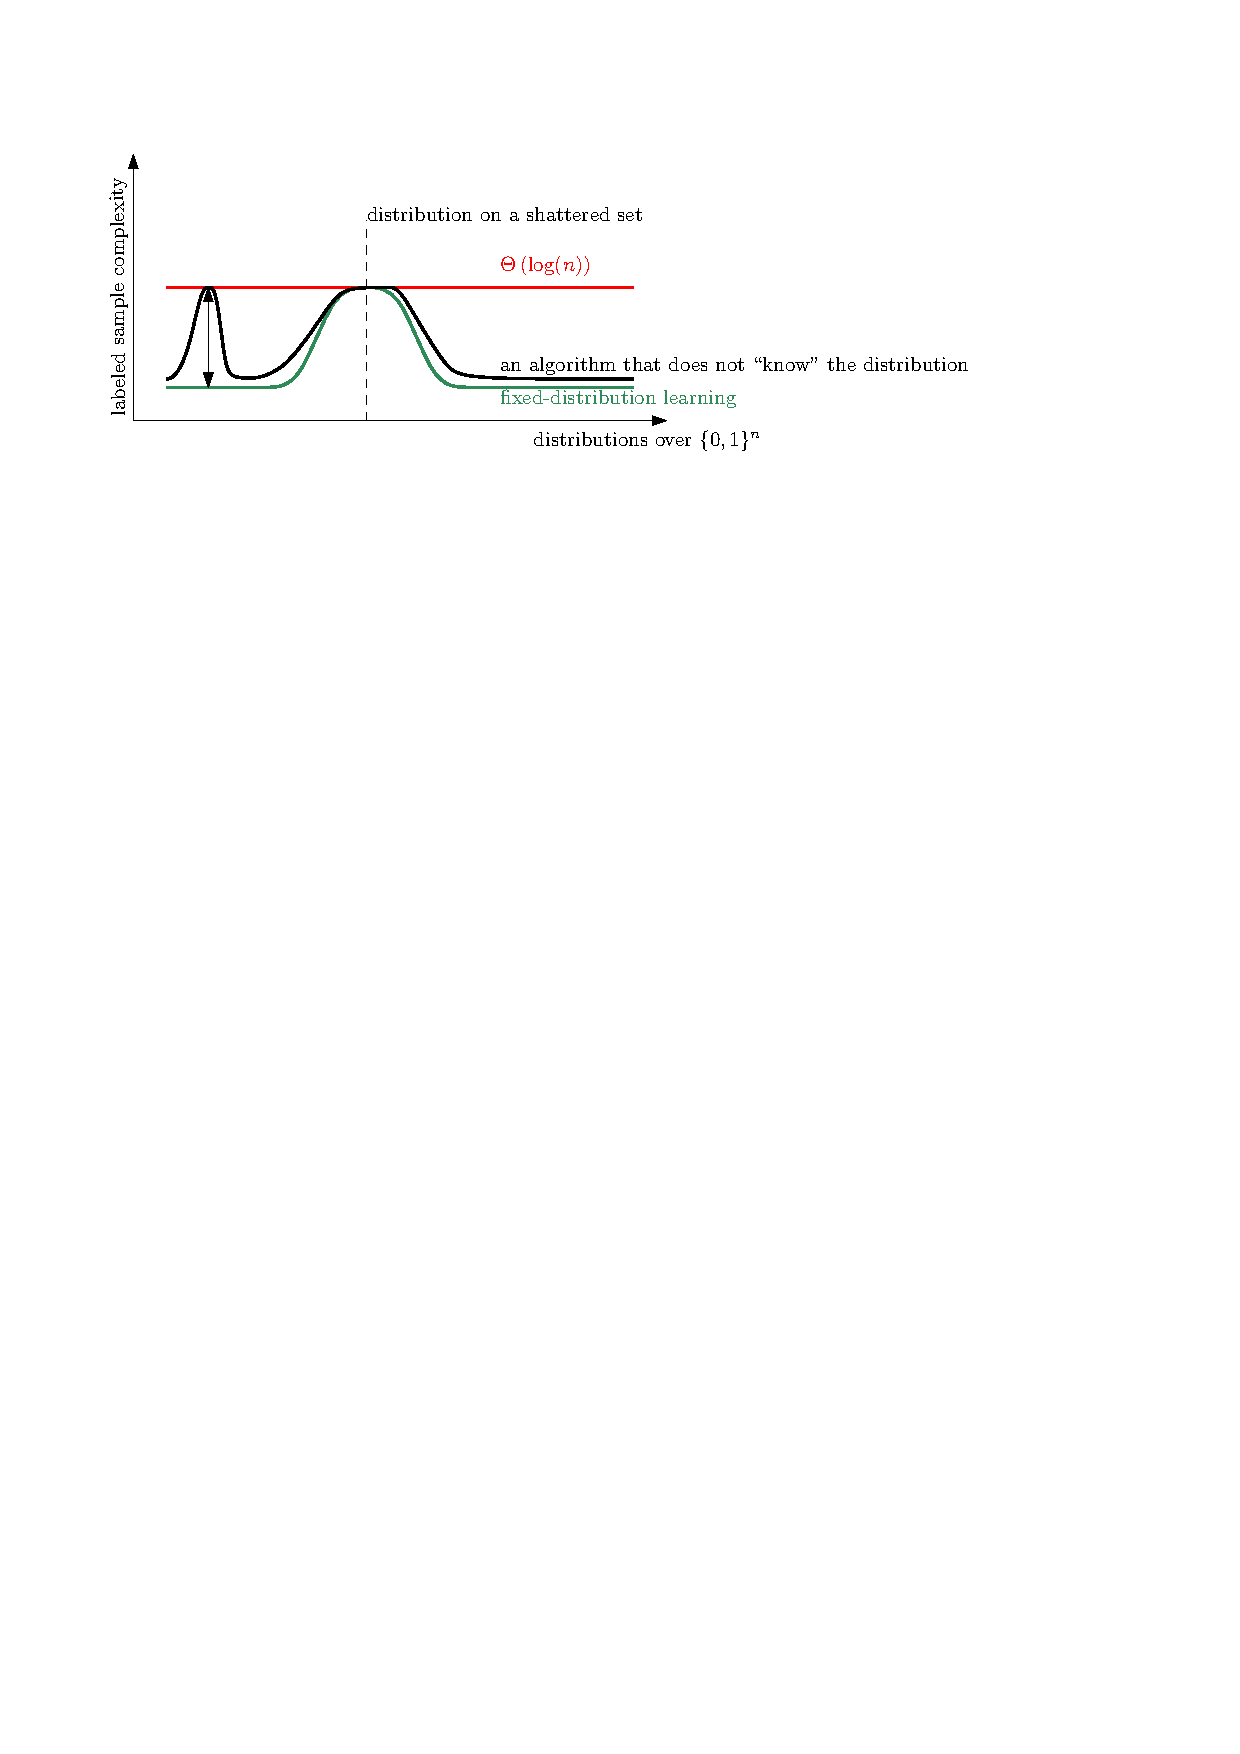
\includegraphics{figure}
\caption{The graph shows sample complexity of learning a class of projections
$C_n$ under various distributions over the domain $\{0,1\}^n$. We assume that
$\epsilon$ and $\delta$ are constant; e.g. $\epsilon = \delta = 0.1$. The graph
shows three lines. The red horizontal line is the optimal PAC sample complexity for class of
projections, which is $\Theta(VC(C_n)) = \Theta(\log_2 n)$. The green line corresponds to
the optimal sample complexity for fixed-distribution learning, i.e., the learning where algorithm ``knows''
(``is tailored to'') the specific distribution. The green line touches the red
line for certain distributions, but is lower for other distributions.
In particular, for certain distributions the green line is $O(1)$.
The black line is the sample complexity for an arbitrary fixed algorithm
that does \emph{not} receive the distribution as input. (For example, the reader can think of the ERM
algorithm.) Obviously, the black line must lie above the green line. In this paper,
we prove that there exist a distribution where the black line is $\Omega(\log
n)$ times higher than green line.}
\label{figure:sample-complexity}
\end{figure}

\section{Preliminaries}

We denote by $C_n$ the class of projections over the domain $\{0,1\}^n$. The
class $C_n$ consists of $n$ functions $c_1, c_2, \dots, c_n$ from $\{0,1\}^n$ to
$\{0,1\}$. For any $i \in \{1,2,\dots,n\}$, for any $x \in \{0,1\}^n$,
the function $c_i$ is defined as $c_i((x[1], x[2], \dots, x[n])) = x[i]$.
The Vapnik-Chervonenkis dimension of $C_n$ is $d = \lfloor \log_2 n \rfloor$; see
Proposition~\ref{proposition:vc-dimension-projections} below.

\begin{proposition}
\label{proposition:vc-dimension-projections}
Vapnik-Chervonenkis dimension of $C_n$ is $\lfloor \log_2 n \rfloor$.
\end{proposition}

\begin{proof}
Vapnik-Chervonenkis dimension is the size of the largest shattered set; let us
denote it by $d$. Let $S$ be a shattered set of size $d$. Then, there must be at
least $2^d$ distinct functions in $C_n$. Hence, $d \le \log_2 |C_n| =
\log_2 n$. Since $d$ is an integer, we conclude that $d \le \lfloor \log_2 n
\rfloor$.

On the other hand, we construct a shattered set of size $\lfloor \log_2 n
\rfloor$. The set will consists of points $x_1, x_2, \dots, x_{\lfloor \log_2 n
\rfloor} \in \{0,1\}^n$. For any $i \in \{1,2,\dots,\lfloor \log_2 n \rfloor\}$
and any $j \in \{0,1,2,\dots,n-1\}$, we define $x_i[j]$ to be the $i$-th bit of the
in the binary representation of the number $j$. (The bit at position $i=1$ is the
least significant bit.) It is not hard to see that for any $v \in
\{0,1\}^{\lfloor \log_2 n \rfloor}$, there exists $c \in C_n$ such that $v =
(c(x_1), c(x_2), \dots, c(x_{\lfloor \log_2 n \rfloor}))$. Indeed, given $v$,
let $k \in \{0,1,\dots,2^{\lfloor \log_2 n \rfloor} - 1\}$ be the number with
binary representation $v$, then we can take $c = c_{k+1}$.
\end{proof}

The family $\P_n$ consists of $n!$ probability distributions over
$\{0,1\}^n$. For any permutation $\sigma \in S_n$, we define a probability distribution
$P_{\sigma}$ over $\{0,1\}^n$. To describe the distribution $P_\sigma$, let $X = (X[1],
X[2], \dots, X[n])$ be a random vector drawn from $P_\sigma$.
The distribution $\P_\sigma$ is a product distribution,
i.e., $\Pr[X = x] = \prod_{j=1}^n \Pr_{X}[X[j] = x[j]]$
for any $x \in \{0,1\}^n$. The marginal distributions
of the coordinates are
$$
\Pr[X[\sigma(j)] = 1] = p_j = \frac{1}{\log_2(3 + j)} \qquad \qquad \text{for $j=1,2,\dots,n$} \; .
$$

\begin{theorem}[Fixed distribution learning]
For any $\epsilon > 0$ and any distribution from $P \in \P_n$,
there exists an algorithm such that for any $\delta > 0$
the algorithm $\epsilon$-learns any target function
from $C_n$ from $O \left( \frac{\log(1/\delta)}{\epsilon^2} \right)$
examples with probability at least $1 - \delta$.
\end{theorem}

\begin{proof}
The proof relies on a result of \cite{Benedek-Itai-1991} for learning under
``fixed'' distributions. If $P$ is any probability distribution on some domain,
then $d_P(f,g) = \Pr_{X \sim P}[f(X) \neq g(X)]$ is a pseudo-metric on the set of all
$\{0,1\}$-valued functions on the domain. \cite{Benedek-Itai-1991} proved that
if a $C$ class of $\{0,1\}$-functions has an $\frac{\epsilon}{2}$-cover of size
$N$, then any target from $C$ is $\epsilon$-learnable from $O
\left( \frac{\log N + \log (1/\delta)}{\epsilon}\right)$ examples
with probability at least $1-\delta$.

We show that for any distribution in $\P_n$ the class $C_n$ has an $\frac{\epsilon}{2}$-cover of size
$N = \max\{3, \lceil 2^{4/\epsilon}\rceil  - 2 \}$. This will imply the lemma.

Consider distribution $P_{\sigma} \in \P_n$ for some $\sigma \in S_n$.
We claim that $C_{\epsilon/2} = \{ c_{\sigma(1)},
c_{\sigma(2)}, \dots, c_{\sigma(N)} \}$ is an $\frac{\epsilon}{2}$-cover of
$C_n$. That is, we claim that for any $c \in C_n$, there exists $c' \in
C_{\epsilon/2}$ such that $d_{P_{\sigma}}(c,c') \le \epsilon/2$.

Any $c \in C_n$ is of the form $c = c_{\sigma(k)}$ for some $k \in \{1,2,\dots,n\}$.
If $k \le N$ then $c_{\sigma(k)}$ lies in $C_{\epsilon/2}$ and thus, trivially, $d_{P_{\sigma}}(c_{\sigma(k)},c_{\sigma(k)}) = 0$.
Otherwise, if  $k \ge N + 1$,
\begin{align*}
d_{P_{\sigma}}(c_{\sigma(N)}, c_{\sigma(k)})
& = \Pr_{X \sim P_{\sigma}}[X_{\sigma(N)} \neq X_{\sigma(k)} ] \\
& = p_N (1 - p_k) + p_k (1 - p_N) \\
& \le p_N + p_k \\
& \le 2 p_N \\
& \le \frac{2}{\log_2(2 + N)} \\
& \le \epsilon/2 \; .
\end{align*}
\end{proof}

For any function $h:\{0,1\}^n \to \{0,1\}$ any permutation $\sigma \in S_n$, any
projection $i \in \{1,2,\dots,n\}$, define
$$
\err_{\sigma,i}(h) = \Pr_{X \sim P_{\sigma}}[h(X) \neq c_i(X)] \; .
$$
In other words, $\err_{\sigma,i}$ is the error of $h$ with respect to the target
$c_i$ under the distribution $P_{\sigma}$.

\begin{theorem}[Learning without knowledge of the distribution]
For any algorithm $A$ there exists a distribution $P \in \P_n$
and a target concept $c \in C_n$ that requires at least $\Omega \left(??? \right)$
labeled examples to $\epsilon$-learn with probability at least $1 - \delta$.
\end{theorem}

\begin{proof}
Let $A$ be any (possibly improper) learning algorithm. We formalize it is as a function
$$
A:\bigcup_{m=0}^\infty\{0,1\}^{m \times n} \times \{0,1\})^m \to \{0,1\}^{\{0,1\}^n} \; .
$$
The algorithm receives an $m \times n$ matrix and a binary vector of length $m$.
The rows of the matrix corresponds to unlabeled examples and the vector encodes
the labels. The output of the $A$ is any function from $\{0,1\}^n \to \{0,1\}$.

Fix the number of examples $m$ to be any non-negative less than $\log n$. We
demostrate the existence of a pair $(P,c) \in \P_n \times C_n$ by probabilistic
method. Let $\sigma$ be uniformly random permutation over $\{1,2,\dots,n\}$. Let
$J = \sigma(1)$ and note that $J$ is uniformly distributed over
$\{1,2,\dots,n\}$. We will show that if we feed $A$ an i.i.d. sample of size $m$
from $P_\sigma$ labeled according to $c_J$, with probability at least $\delta$
the error of the algorithm is at least $\epsilon$. This will imply the existence
of the pair $(P,c)$.

Formally, let $X_1, X_2, \dots, X_m$ be an i.i.d. sample from $P_{\sigma}$ and
let $Y_1 = c_J(X_1), Y_2 = c_J(X_2), \dots, Y_m = c_J(X_m)$ be the target
labels. Let $X$ be $m \times n$ matrix with entries $X_i[j]$ and let $Y = (Y_1,
Y_2, \dots, Y_m)$ be the vector of labels. The output of the algorithm is $A(X,Y)$.
We will show that
\begin{equation}
\label{equation:failure-probability}
\Pr \left[\err_{\sigma,J}(A(X,Y)) \ge \epsilon \right] \ge \delta \; .
\end{equation}
Since $\Pr \left[\err_{\sigma,J}(A(X,Y)) \ge \epsilon \right] = \Exp\left[ \Pr \left[\err_{\sigma,J}(A(X,Y)) \ge \epsilon \, \middle| \, \sigma, J \right] \right]$
the inequality \eqref{equation:failure-probability} implies that there
exists $\sigma \in S_n$ and $j \in \{1,2,\dots,n\}$ such that under the
distribution $P_\sigma$, the algorithm $A$ fails to $\epsilon$-learn the target
$c_j$ with probability at least $\delta$.

To prove \eqref{equation:failure-probability}, we first introduce necessary
notation. For any $n \times m$ matrix $B$, let $B[1], B[2], \dots, B[n]$ be its
columns and let $c(B) = \{ j \in \{1,2,\dots, n\} ~|~ \ B[j] = B[1] \}$ be the set
of indices of columns matching the first column. Note that $1 \in c(B)$. For any
subset $K \subseteq \{1,2,\dots,n\}$, we define $p(K) = \sum_{j \in K} p_j$
where $p_j = 1/\log_2(3 + j)$. For any set $K \subseteq \{1,2,\dots,n\}$, let
$S_n(K) = \{ \pi \in S_n ~:~ \forall j \in \{1,2,\dots,n\} \setminus K, \ \pi(j) =
j \}$ be the set of permutations of $\{1,2,\dots,n\}$ that keeps the elements in
$K$ in place. There are $|K|!$ permutations in $S_n(K)$. For any permutation $\pi \in S_n$
and any $m \times n$ matrix $B$, let $\pi(B)$ an $m \times n$ matrix
$$
\pi(B) = \left[ B[\pi(1)], B[\pi(2)], \dots, B[\pi(n)] \right]
$$
with columns permuted according to $\pi$.

Let $M$ be $m \times n$ binary matrix $M = \sigma(X)$. Note that
$$
\Pr[M_{i,j} = 1] = \Pr[X_i[\sigma(j)] = 1] = p_j \qquad \qquad \text{for $i=1,2,\dots,m$, \ $j=1,2,\dots,n$}
$$
and that the entries of $M$ are independent. Also, note that $M$ and $\sigma$
are independent.

Let $\alpha$ be randomly chosen from $S_n(c(M))$. Note that $\sigma$ and
$\alpha$ are independent. Somewhat less obviously, $\alpha \circ \sigma$ and $M$
are independent and thus $(M,\sigma)$ and $(M, \alpha \circ \sigma)$ have the
same distribution; this is due to the fact that conditioned on $M$ and $\alpha$,
both $\sigma$ and $\alpha \circ \sigma$ have uniform distribution over $S_n$.

Since $X = \sigma^{-1}(M)$ and $M = \alpha(M) = \alpha^{-1}(M)$ and $Y = X[J] = X[\sigma(1)] = M[1]$,
\begin{align*}
& \Pr \left[ \err_{\sigma,J}(A(X,Y)) \ge \epsilon \right] \\
& = \Pr \left[ \err_{\sigma,\sigma(1)}(A(\sigma^{-1}(M), M[1])) \ge \epsilon \right] \\
& = \Pr \left[ \err_{\alpha \circ \sigma,\alpha(\sigma(1))}(A(\sigma^{-1} (\alpha^{-1}(M)), M[1])) \ge \epsilon \right] \\
& = \Pr \left[ \err_{\alpha \circ \sigma,\alpha(\sigma(1))}(A(\sigma^{-1}(M), M[1])) \ge \epsilon \right] \\
& \ge \Pr \left[ p(c(M)) \ge \tfrac{1}{2} + \epsilon \ \wedge \ \err_{\alpha \circ \sigma,\alpha(\sigma(1))}(A(\sigma^{-1}(M), M[1])) \ge \epsilon \right] \\
& = \sum_{\substack{\pi \in S_n \\ B \in \{0,1\}^{n \times m} \\ p(c(B)) \ge \frac{1}{2} + \epsilon}} \Pr \left[ \sigma = \pi \ \wedge \ M = B  \ \wedge \ \err_{\alpha \circ \pi,\alpha(\pi(1))}(A(\pi^{-1}(B), B[1])) \ge \epsilon \right] \\
& = \sum_{\substack{\pi \in S_n \\ B \in \{0,1\}^{n \times m} \\ p(c(B)) \ge \frac{1}{2} + \epsilon}} \Pr \left[ \err_{\alpha \circ \pi,\alpha(\pi(1))}(A(\pi^{-1}(B), B[1])) \ge \epsilon \, \middle| \, M = B \wedge \sigma = \pi \right] \cdot \Pr[M = B] \cdot \Pr[\sigma = \pi]
\end{align*}
Fix a matrix $B \in \{0,1\}^{n \times m}$ and a permutation $\pi \in S_n$. Conditioned on $M = B$ and $\sigma = \pi$,
$\alpha$ is uniformly distributed on $S_n(B)$ and $h = A(\pi^{-1}(B), B[1])$ is a fixed non-random classifier.
We compute
\begin{align*}
\Exp \left[ \err_{\alpha \circ \pi,\alpha(\pi(1))}(h) \, \middle| \, M = B \wedge \sigma = \pi \right]
& = \frac{1}{|c(B)|!} \sum_{\alpha \in S_n(B)} \err_{\alpha \circ \pi,\alpha(\pi(1))}(h) \\
& = \frac{1}{|c(B)|!} \sum_{\alpha \in S_n(B)} \Pr_{Z \sim P_{\alpha \circ \pi}} \left[ h(Z) \neq c_{\alpha(\pi(1))}(Z) \right] \\
\end{align*}

\end{proof}

\section{Junk}

A permutation $\pi \in S_n$ is said to be a swap of $i,j$
if $\pi(i) = j$ and $\pi(j) = i$ and for all $k \in \{1,2,\dots,n\} \setminus \{i,j\}$
$\pi(k) = k$.

\begin{lemma}
\label{lemma:projection-distances}
Let $i \in \{2,3,\dots,n\}$. Let $\alpha \in S_n$ be a swap of $1$ and $i$.
Let $a,b \in \{0,1\}^n$ be binary vectors such that $a_i \neq b_i$
and $a_j = b_j$ for all $j \in \{1,2,\dots,n\} \setminus \{i\}$.
Let $h:\{0,1\}^n \to \{0,1\}$ be an arbitary function. Then, for any permutation $\sigma \in S_n$,
$$
\err_{c_{\sigma(1)},P_{\sigma,a}}(h) + \err_{c_{\sigma(1)},P_{\sigma,b}}(h) +
\err_{c_{\sigma(\alpha(1))},P_{\sigma \circ \alpha,b}}(h) + \err_{c_{\sigma(\alpha(1))},P_{\sigma \circ \alpha,b}}(h) \ge 1 \; .
$$
\end{lemma}

\begin{proof}
We claim that for any $x \in \{0,1\}^n$,
\begin{equation}
\label{equation:probability-ratio}
\frac{\displaystyle
\min \left\{ \Pr_{X \sim P_{\sigma,a}}[X = x] + \Pr_{X \sim P_{\sigma,b}}[X = x], \ \Pr_{X \sim P_{\sigma \circ \alpha,a}}[X = x] + \Pr_{X \sim P_{\sigma \circ \alpha,b}}[X = x] \right\}}{
\displaystyle \Pr_{X \sim P_{\sigma,a}}[X = x] + \Pr_{X \sim P_{\sigma,b}}[X = x] + \Pr_{X \sim P_{\sigma \circ \alpha,b}}[X = x] + \Pr_{X \sim P_{\sigma \circ \alpha,b}}[X = x]}
= \frac{1}{2} \; .
\end{equation}
Since $P_{\sigma,a}$,
$P_{\sigma,b}$, $P_{\sigma \circ \alpha,a}$, $P_{\sigma \circ \alpha,b}$
are product distributions and the marginal distributions of $X_{\sigma(k)}$
for any $k \not \in \{1,i\}$ under these four distributions are the same,
after cancelling common terms, we can write the fraction on the left side as $A/B$ where
\begin{multline*}
A =
\min \left\{ \Pr_{X \sim P_{\sigma,a}}[X_{\sigma(1)} = x_{\sigma(1)} \wedge X_{\sigma(i)} = x_{\sigma(i)}]
+ \Pr_{X \sim P_{\sigma,b}}[X_{\sigma(1)} = x_{\sigma(1)} \wedge X_{\sigma(i)} = x_{\sigma(i)}],  \right. \\
\left. \Pr_{X \sim P_{\sigma \circ \alpha,a}}[X_{\sigma(1)} = x_{\sigma(1)} \wedge X_{\sigma(i)} = x_{\sigma(i)}]
+ \Pr_{X \sim P_{\sigma \circ \alpha,b}}[X_{\sigma(1)} = x_{\sigma(1)} \wedge X_{\sigma(i)} = x_{\sigma(i)}]  \right\}
\end{multline*}
and
\begin{multline*}
B =
\Pr_{X \sim P_{\sigma,a}}[X_{\sigma(1)} = x_{\sigma(1)} \wedge X_{\sigma(i)} = x_{\sigma(i)}] + \Pr_{X \sim P_{\sigma,b}}[X_{\sigma(1)} = x_{\sigma(1)} \wedge X_{\sigma(i)} = x_{\sigma(i)}] \\
+ \Pr_{X \sim P_{\sigma \circ \alpha,a}}[X_{\sigma(1)} = x_{\sigma(1)} \wedge X_{\sigma(i)} = x_{\sigma(i)}] + \Pr_{X \sim P_{\sigma \circ \alpha,b}}[X_{\sigma(1)} = x_{\sigma(1)} \wedge X_{\sigma(i)} = x_{\sigma(i)}] \; .
\end{multline*}
Since $a_i \neq b_i$,
$$
\Pr_{X \sim P_{\sigma,a}}[X_{\sigma(1)} = x_{\sigma(1)} \wedge X_{\sigma(i)} = x_{\sigma(i)}] + \Pr_{X \sim P_{\sigma,b}}[X_{\sigma(1)} = x_{\sigma(1)} \wedge X_{\sigma(i)} = x_{\sigma(i)}] =
\Pr_{X \sim P_{\sigma,a}}[X_{\sigma(1)} = x_{\sigma(1)}] = \frac{1}{2}
$$
and
$$
\Pr_{X \sim P_{\sigma \circ \alpha,a}}[X_{\sigma(1)} = x_{\sigma(1)} \wedge X_{\sigma(i)} = x_{\sigma(i)}] + \Pr_{X \sim P_{\sigma \circ \alpha,b}}[X_{\sigma(1)} = x_{\sigma(1)} \wedge X_{\sigma(i)} = x_{\sigma(i)}] =
\Pr_{X \sim P_{\sigma \circ \alpha,a}}[X_{\sigma(i)} = x_{\sigma(i)}] = \frac{1}{2} \; .
$$

\allowdisplaybreaks
Equipped with \eqref{equation:probability-ratio} we finish the proof of the lemma:
\begin{align*}
& \err_{c_{\sigma(1)},P_{\sigma,a}}(h) + \err_{c_{\sigma(1)},P_{\sigma,b}}(h) + \err_{c_{\sigma(\alpha(1))},P_{\sigma \circ \alpha,b}}(h) + \err_{c_{\sigma(\alpha(1))},P_{\sigma \circ \alpha,b}}(h) \\
& = \err_{c_{\sigma(1)},P_{\sigma,a}}(h) + \err_{c_{\sigma(1)},P_{\sigma,b}}(h) + \err_{c_{\sigma(i)},P_{\sigma \circ \alpha,a}}(h) + \err_{c_{\sigma(i)},P_{\sigma \circ \alpha,b}}(h) \\
& = \Pr_{X \sim P_{\sigma,a}}[h(X) \neq X_{\sigma(1)}] + \Pr_{X \sim P_{\sigma,b}}[h(X) \neq X_{\sigma(1)}] + \Pr_{X \sim P_{\sigma \circ \alpha,b}}[h(X) \neq X_{\sigma(i)}] + \Pr_{X \sim P_{\sigma \circ \alpha,b}}[h(X) \neq X_{\sigma(i)}] \\
& = \sum_{x \in \{0,1\}^n} \Pr_{X \sim P_{\sigma,a}}[X = x \wedge h(x) \neq x_{\sigma(1)}] + \Pr_{X \sim P_{\sigma,b}}[X = x \wedge h(x) \neq x_{\sigma(1)}] \\
  & \qquad \qquad + \Pr_{X \sim P_{\sigma \circ \alpha,a}}[X = x \wedge h(x) \neq x_{\sigma(i)}] + \Pr_{X \sim P_{\sigma \circ \alpha,b}}[X = x \wedge h(x) \neq x_{\sigma(i)}] \\
& \ge \sum_{\substack{x \in \{0,1\}^n \\ x_{\sigma(1)} \neq x_{\sigma(i)}}} \Pr_{X \sim P_{\sigma,a}}[X = x \wedge h(x) \neq x_{\sigma(1)}] + \Pr_{X \sim P_{\sigma,b}}[X = x \wedge h(x) \neq x_{\sigma(1)}] \\
& \qquad \qquad + \Pr_{X \sim P_{\sigma \circ \alpha,a}}[X = x \wedge h(x) \neq x_{\sigma(i)}] + \Pr_{X \sim P_{\sigma \circ \alpha,b}}[X = x \wedge h(x) \neq x_{\sigma(i)}]  \\
& \ge \sum_{\substack{x \in \{0,1\}^n \\ x_{\sigma(1)} \neq x_{\sigma(i)}}} \min \left\{ \Pr_{X \sim P_{\sigma,a}}[X = x] + \Pr_{X \sim P_{\sigma,b}}[X = x], \ \Pr_{X \sim P_{\sigma \circ \alpha,a}}[X = x] + \Pr_{X \sim P_{\sigma \circ \alpha,b}}[X = x] \right\}
  \displaybreak[4] \\
& = \sum_{\substack{x \in \{0,1\}^n \\ x_{\sigma(1)} \neq x_{\sigma(i)}}} \frac{1}{2} \left(
\Pr_{X \sim P_{\sigma,a}}[X = x] + \Pr_{X \sim P_{\sigma,b}}[X = x] + \Pr_{X \sim P_{\sigma \circ \alpha,a}}[X = x] + \Pr_{X \sim P_{\sigma \circ \alpha,b}}[X = x] \right) \\
& = \frac{1}{2} \left( \Pr_{X \sim P_{\sigma,a}}[X_{\sigma(1)} \neq X_{\sigma(i)}] + \Pr_{X \sim P_{\sigma,b}}[X_{\sigma(1)} \neq X_{\sigma(i)}]
+ \Pr_{X \sim P_{\sigma \circ \alpha,a}}[X_{\sigma(1)} \neq X_{\sigma(i)}] + \Pr_{X \sim P_{\sigma \circ \alpha,b}}[X_{\sigma(1)} \neq X_{\sigma(i)}] \right) \\
& = \frac{1}{2} \left( \frac{1}{2} + \frac{1}{2} + \frac{1}{2} + \frac{1}{2} \right) = 1 \; .
\end{align*}
The first inequality is trivial. The second inequality follows from the fact that
if $x_{\sigma(1)} \neq x_{\sigma(i)}$ then $h(x)$ must be equal to either $x_{\sigma(1)}$ or $x_{\sigma(i)}$.
\end{proof}



\section{Realizable Case: Monotone Disjuctions}

Consider the class $C_n$ of monotone disjuctions over $D_n = \{0,1\}^n$.
There are $2^n$ functions in $C_n$. For each subset $I \subseteq \{1,2,\dots,n\}$
there is monotone disjuction $c_I:D_n \to \{0,1\}$ defined by
$$
c_I(x) = \bigvee_{i \in I} x_i \; .
$$
We define $c_\emptyset$ to be constant zero function.

We consider the same family of distributions $\P_n$ as in the previous section.
Let $P = P_{Identity} \in \P_n$. We compute the distance $d_P(c_I, c_J)$
between any two monotone disjuctions. For any subset
$K \subseteq \{1,2,\dots,n\}$, let $A_K$ be the event that all for all $i \in K$, $x_i = 0$.
\begin{align*}
d_P(c_I, c_J)
& = \Pr_{x \sim P}[c_I(x) \neq c_J(x)] \\
& = \Pr_{x \sim P}[A_{I \cap J} \wedge ((A_{I \setminus J} \wedge \overline{A_{J \setminus I}}) \vee (\overline{A_{I \setminus J}} \wedge A_{J \setminus I} )) ] \\
& = \Pr[A_{I \cap J}] \cdot \left\{ \Pr[A_{I \setminus J}] (1 - \Pr[A_{J \setminus I}]) + (1 - \Pr[A_{I \setminus J}]) \Pr[A_{J \setminus I}] \right\} \\
& = \Pr[A_{I \cap J}] \cdot \left\{ \Pr[A_{I \setminus J}] + \Pr[A_{J \setminus I}] - 2 \Pr[A_{I \setminus J}] \Pr[A_{J \setminus I}] \right\} \\
& = \Pr[A_I] + \Pr[A_J] - 2 \Pr[A_{I \cup J}] \\
& = \prod_{i \in I} (1 - p_i) + \prod_{j \in J} (1 - p_j) - 2 \prod_{k \in I \cup J} (1 - p_k) \; . \\
\end{align*}

\section{Agnostic Model}

Let $C$ be a concept class over a domain $X$. Let $P$ be any distribution over
$X$. We define the ``disagreement'' pseudometric $d_P(c,c') = \Pr_{(x,y) \sim
P}[c(x) = c'(x)]$ on $C$. We denote by $N(C,P,\epsilon,)$ be the size of the
smallest $\epsilon$-cover of $C$ with respect to $d_P$.

Let $R(c) = \Pr_{(x,y) \sim P}[c(x) \neq y]$ be the risk.
For an i.i.d. sample $(X_1, Y_1), \dots, (X_n, Y_n)$ be an i.i.d. sample
from $P$, we define the empirical risk
$$
R_n(c) = \sum_{i=1}^n \indicator{c(X_i) \neq Y_i} \; .
$$
Finally, let $c_n = \argmin_{c \in C} R_n(c)$.

\bibliography{biblio}
\bibliographystyle{plainnat}

\end{document}
